\graphicspath{{appendices/appendix_1/figures/}}
\chapter{Appendix 1}

\section{ITS2 Sequencing}
\label{sec:app_its2}

\subsection{PCR Gels}
\begin{figure}[H]
    \centering
    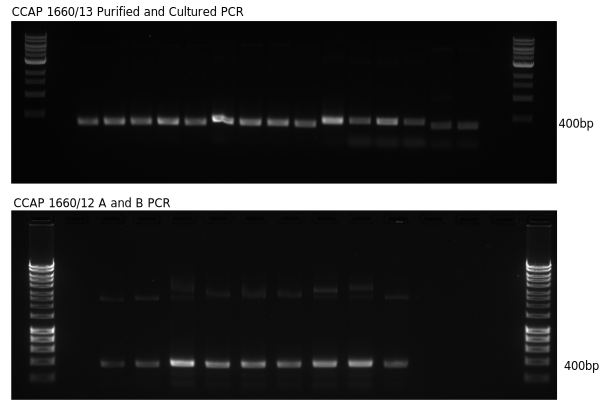
\includegraphics[width=\textwidth]{ITS2_PCR_gels.pdf}
    \caption[Gel images of ITS2 PCR from CCAP1660/12 and CCAP1660/13 reactions]{
        Gel image of the PCR products from initial ITS2 PCR in CCAP1660/12 initial reactions (1660/12 1-20) 
as well as CCAP1660/13 purified and culture reactions. As all PCR products were within expected
size range of 400bp products were pooled for cloning. No gel pictures are available for other reactions.} 
\label{fig:endo_annot}
\end{figure}

\subsection{ITS2 Sequences}


\resizebox{\textwidth}{!}{\begin{filecontents*}{appendices/appendix_1/figures/its2_sequences.fas}
>1660_12_1
TGCAGAATTCCGTGAACCATCGAATCTTTGAACGCAAATTGCGCCCGAGGCTTCGGCCGAGGGCATGTCTGCCTCAGCGTCGGCTTACCCCCTCGCCTCCCCTTCACCGGGTGAGTGCGGATCTGGCCCTCCCGGCTCCGACTGAACTCGTTCAGCCATCCGGGTCGGCTGAAGTGCAGAGGCTTGAGCATGGACCCCGTTTGCAGGGCAATGGCTTGGTAGGTAGCATTGCTACGCAGCCTGCCGTCGCCCGAGGGGCCTTTGCTGGCGGCCCAGCAGGAACCGGGGCGTCAAACCTCCGGCGTCTCACACTTTCGACCTGAGCTCAGGCAAGATTACCCGCTGAACTTAAGCATATCAATAAGCAGAGGAAAATAAACTAACTAGGATGCCCTTAGTAACGGCGAGCGAACCGGGCAAAGCCCAACTTGAAAATCTCCAGCCTCC
>1660_12_2
TGCAGAATTCCGTGAACCATCGAATCTTTGAACGCAAATTGCGCCCGAGGCTTCGGCCGAGGGCATGTCTGCCTCAGCGTCGGCTTACCCCCTCGCCTCCCCTTCACCGGGTGAGTGCGGATCTGGCCCTCCCGGCTCCGACTGAACTCGTTCAGCCATCCGGGTCGGCTGAAGTGCAGAGGCTTGAGCATGGACCCCGTTTGCAGGGCAATGGCTTGGTAGGTAGCATTGCTACGCAGCCTGCCGTCGCCCGAGGGGCCTTTGCTGGCGGCCCAGCAGGAACCGGGGCGTCAAACCCCCGGCGTCTCACACTTTCGACCTGAGCTCAGGCAAGATTACCCGCTGAACTTAAGCATATCAATAGGCGGAGGAAAATAAACTAACTAGGATGCCCTTAGTAACGGCGAGCGAACCGGGCAAAGCCCAACTTGAAAATCTCCAGCCTCC
>1660_12_3
TGCAGAATTCCGTGAACCATCGAATCTTTGAACGCAAATTGCGCCCGAGGCTTCGGCCGAGGGCATGTCTGCCTCAGCGTCGGCTTACCCCCTCGCCTCCCCTTCACCGGGTGAGTGCGGATCTGGCCCTCCCGGCTCCGACTGAACTCGTTCAGCCATCCGGGTCGGCTGAAGTGCAGAGGCTTGAGCATGGACCCCGTTTGCAGGGCAATGGCTTGGTAGGTAGCATTGCTACGCAGCCTGCCGTCGCCCGAGGGGCCTTTGCTGGCGGCCCAGCAGGAACCGGGGCGTCAAACCCCCGGCGTCTCACACTTTCGACCTGAGCTCAGGCAAGATTACCCGCTGAACTTAAGCATATCAATAAGCGGAGGAAAATAAACTAACTAGGATGCCCTTAGTAACGGCGAGCGAACCGGGCAAAGCCCAACTTGAAAATCTCCAGCCTCC
>1660_12_6
TGCAGAATTCCGTGAACCATCGAATCTTTGAACGCAAATTGCGCCCGAGGCTTCGGCCGAGGGCATGTCTGCCTCAGCGTCGGCTTACCCCCTCGCCTCCCCTTCACCGGGTGAGTGCGGATCTGGCCCTCCCGGCTCCGGCTGAACTCGTTCAGCCATCCGGGTCGGCTGAAGTGCAGAGGCTTGAGCATGGACCCCGTTTGCAGGGCAATGGCTTGGTAGGTAGCATTGCTACGCAGCCTGCCGTCGCCCGAGGGGCCTTTGCTGGCGGCCCAGCAGGAACCGGGGCGTCAAACCTCCGGCGTCTCACACTTTCGACCTGAGCTCAGGCAAGATTACCCGCTGAACTTAAGCATATCAATAAGCAGAGGAAAATAAACTAACTAGGATGCCCTTAGTAACGGCGAGCGAACCGGGCAAAGCCCAACTTGAAAATCTCCAGCCTCC
>1660_12_6rev
TGCAGAATTCCGTGAACCATCGAATCTTTGAACGCAAATTGCGCCCGAGGCTTCGGCCGAGGGCATGTCTGCCTCAGCGTCGGCTTACCCCCTCGCCTCCCCTTCACCGGGTGAGTGCGGATCTGGCCCTCCCGGCTCCGGCTGAACTCGTTCAGCCATCCGGGTCGGCTGAAGTGCAGAGGCTTGAGCATGGACCCCGTTTGCAGGGCAATGGCTTGGTAGGTAGCATTGCTACGCAGCCTGCCGTCGCCCGAGGGGCCTTTGCTGGCGGCCCAGCAGGAACCGGGGCGTCAAACCTCCGGCGTCTCACACTTTCGACCTGAGCTCAGGCAAGATTACCCGCTGAACTTAAGCATATCAATAAGCAGAGGAAAATAAACTAACTAGGATGCCCTTAGTAACGGCGAGCGAACCGGGCAAAGCCCAACTTGAAAATCTCCAGCCTCC
>1660_12_8
TGCAGAATTCCGTGAACCATCGAATCTTTGAACGCAAATTGCGCCCGAGGCTTCGGCCGAGGGCATGTCTGCCTCAGCGTCGGCTTACCCCCTCGCCTCCCCTTCACCGGGTGAGTGCGGATCTGGCCCTCCCGGCTCCGACTGAACTCGTTCAGCCATCCGGGTCGGCTGAAGTGCAGAGGCTTGAGCATGGACCCCGTTTGCAGGGCAATGGCTTGGTAGGTAGCATTGCTACGCAGCCTGCCGTCGCCCGAGGGGCCTTTGCTGGCGGCCCAGCAGGAACCGGGGCGTCAAACCCCCGGCGTCTCACACTTTCGACCTGAGCTCAGGCAAGATTACCCGCTGAACTTAAGCATATCAATAAGCGGAGGAAAATAAACTAACTAGGATGCCCTTAGTAACGGCGAGCGAACCGGGCAAAGCCCAACTTGAAAATCTCCAGCCTCC
>1660_12_9
TGCAGAATTCCGTGAACCATCGAATCTTTGAACGCAAATTGCGCCCGAGGCTTCGGCCGAGGGCATGTCTGCCTCAGCGTCGGCTTACCCCCTCGCCTCCCCTTCACCGGGTGAGTGCGGATCTGGCCCTCCCGGCTCCGACTGAACTCGTTCAGCCATCCGGGTCGGCTGAAGTGCAGAGGCTTGAGCATGGACCCCGTTTGCAGGGCAATGGCTTGGTAGGTAGCATTGCTACGCAGCCTGCCGTCGCCCGAGGGGCCTTTGCTGGCGGCCCAGCAGGAACCGGGGCGTCAAACCTCCGGCGTCTCACACTTTCGACCTGAGCTCAGGCAAGATTACCCGCTGAACTTAAGCATATCAATAAGCAGAGGAAAATAAACTAACTAGGATGCCCTTAGTAACGGCGAGCGAACCGGGCAAAGCCCAACTTGAAAATCTCCAGCCTCC
>1660_12_10
TGCAGAATTCCGTGAACCATCGAATCTTTGAACGCAAATTGCGCCCGAGGCTTCGGCCGAGGGCATGTCTGCCTCAGCGTCGGCTTACCCCCTCGCCTCCCCTTCACCGGGTGAGTGCGGATCTGGCCCTCCCGGCTCCGACTGAACTCGTTCAGCCATCCGGGTCGGCTGAAGTGCAGAGGCTTGAGCATGGACCCCGTTTGCAGGGCAATGGCTTGGTAGGTAGCATTGCTACGCAGCCTGCCGTCGCCCGAGGGGCCTTTGCTGGCGGCCCAGCAGGAACCGGGGCGTCAAACCTCCGGCGTCTCACACTTTCGACCTGAGCTCAGGCAAGATTACCCGCTGAACTTAAGCATATCAATAAGCAGAGGAAAATAAACTAACTAGGATGCCCTTAGTAACGGCGAGCGAACCGGGCAAAGCCCAACTTGAAAATCTCCAGCCTCC
>1660_12_15
TGCAGAATTCCGTGAACCATCGAATCTTTGAACGCAAATTGCGCCCGAGGCTTCGGCCGAGGGCATGTCTGCCTCAGCGTCGGCTTACCCCCTCGCCTCCCCTTCACCGGGTGAGTGCGGATCTGGCCCTCCCGGCTCCGACTGAACTCGTTCAGCCATCCGGGTCGGCTGAAGTGCAGAGGCTTGAGCATGGACCCCGTTTGCAGGGCAATGGCTTGGTAGGTAGCATTGCTACGCAGCCTGCCGTCGCCCGAGGGGCCTTTGCTGGCGGCCCAGCAGGAACCGGGGCGTCAAACCTCCGGCGTCTCACACTTTCGACCTGAGCTCAGGCAAGATTACCCGCTGAACTTAAGCATATCAATAAGCAGAGGAAAATAAACTAACTAGGATGCCCTTAGTAACGGCGAGCGAACCGGGCAAAGCCCAACTTGAAAATCTCCAGCCTCC
>1660_12_16
TGCAGAATTCCGTGAACCATCGAATCTTTGAACGCAAATTGCGCCCGAGGCTTCGGCCGAGGGCATGTCTGCCTCAGCGTCGGCTTACCCCCTCGCCTCCCCTTCACCGGGTGAGTGCGGATCTGGCCCTCCCGGCTCCGACTGAACTCGTTCAGCCATCCGGGTCGGCTGAAGTGCAGAGGCTTGAGCATGGACCCCGTTTGCAGGGCAATGGCTTGGTAGGTAGCATTGCTACGCAGCCTGCCGTCGCCCGAGGGGCCTTTGCTGGCGGCCCAGCAGGAACCGGGGCGTCAAACCCCCGGCGTCTCACACTTTCGACCTGAGCTCAGGCAAGATTACCCGCTGAACTTAAGCATATCAATAAGCGGAGGAAAATAAACTAACTAGGATGCCCTTAGTAACGGCGAGCGAACCGGGCAAAGCCCAACTTGAAAATCTCCAGCCTCC
>1660_12_18
TGCAGAATTCCGTGAACCATCGAATCTTTGAACGCAAATTGCGCCCGAGGCTTGGGCCGAGGGCATGTCTGCCTCAGCGTCGGCTTACCCCCTCGCCTCCCCTTCACCGGGTGAGTGCGGATCTGGCCCTCCCGGCTCCGGCTGAACTCGTTCAGCCATCCGGGTCGGCTGAAGTGCAGAGGCTTGAGCATGGACCCCGTTTGCAGGGCAATGGCTTGGTAGGTAGCATTGCTACGCAGCCTGCCGTCGCCCGAGGGGCCTTTGCTGGCGGCCCAGCAGGAACCGGGGCGTCAAACCTCCGGCGTCTCACACTTTCGACCTGAGCTCAGGCAAGATTACCCGCTGAACTTAAGCATATCAATAAGCAGAGGAAAATAAACTAACTAGGATGCCCTTAGTAACGGCGAGCGAACCGGGCAAAGCCCAACTTGAAAATCTCCAGCCTCC
>1660_12_18rev
TGCAGAATTCCGTGAACCATCGAATCTTTGAACGCAAATTGCGCCCGAGGCTTGGGCCGAGGGCATGTCTGCCTCAGCGTCGGCTTACCCCCTCGCCTCCCCTTCACCGGGTGAGTGCGGATCTGGCCCTCCCGGCTCCGGCTGAACTCGTTCAGCCATCCGGGTCGGCTGAAGTGCAGAGGCTTGAGCATGGACCCCGTTTGCAGGGCAATGGCTTGGTAGGTAGCATTGCTACGCAGCCTGCCGTCGCCCGAGGGGCCTTTGCTGGCGGCCCAGCAGGAACCGGGGCGTCAAACCTCCGGCGTCTCACACTTTCGACCTGAGCTCAGGCAAGATTACCCGCTGAACTTAAGCATATCAATAAGCAGAGGAAAATAAACTAACTAGGATGCCCTTAGTAACGGCGAGCGAACCGGGCAAAGCCCAACTTGAAAATCTCCAGCCTCC
>1660_12_19
TGCAGAATTCCGTGAACCATCGAATCTTTGAACGCAAATTGCGCCCGAGGCTTCGGCCGAGGGCATGTCTGCCTCAGCGTCGGCTTACCTCCTCGCCTCCCCTTCACCGGGTGAGTGCGGATCTGGCCCTCCCGGCTCCGACTGAACTCGTTCAGCCATCCGGGTCGGCTGAAGTGCAGAGGCTTGAGCATGGACCCCGTTTGCAGGGCAATGGCTTGGTAGGTAGCATTGCTACGCAGCCTGCCGTCGCCCGAGGGGCCTTTGCTGGCGGCCCAGCAGGAACCGGGGCGTCAAACCCCCGGCGTCTCACACTTTCGACCTGAGCTCAGGCAAGATTACCCGCTGAACTTAAGCATATCAATAAGCGGAGGAAAATAAACTAACTAGGATGCCCTTAGTAACGGCGAGCGAACCGGGCAAAGCCCAACTTGAAAATCTCCAGCCTCC
>1660_12_19rev
TGCAGAATTCCGTGAACCATCGAATCTTTGAACGCAAATTGCGCCCGAGGCTTCGGCCGAGGGCATGTCTGCCTCAGCGTCGGCTTACCTCCTCGCCTCCCCTTCACCGGGTGAGTGCGGATCTGGCCCTCCCGGCTCCGACTGAACTCGTTCAGCCATCCGGGTCGGCTGAAGTGCAGAGGCTTGAGCATGGACCCCGTTTGCAGGGCAATGGCTTGGTAGGTAGCATTGCTACGCAGCCTGCCGTCGCCCGAGGGGCCTTTGCTGGCGGCCCAGCAGGAACCGGGGCGTCAAACCCCCGGCGTCTCACACTTTCGACCTGAGCTCAGGCAAGATTACCCGCTGAACTTAAGCATATCAATAAGCGGAGGAAAATAAACTAACTAGGATGCCCTTAGTAACGGCGAGCGAACCGGGCAAAGCCCAACTTGAAAATCTCCAGCCTCC
>1660_12_A1
TGCAGAATTCCGTGAACCATCGAATCTTTGAACGCAAATTGCGCCCGAGGCTTCGGCCGAGGGCATGTCTGCCTCAGCGTCGGCTTACCCCCTCGCCTCCCCTTCACCGGGTGAGTGCGGATCTGGCCCTCCCGGCTCCGACTGAACTCGTTCAGCCATCCGGGTCGGCTGAAGTGCAGAGGCTTGAGCATGGACCCCGTTTGCAGGGCAATGGCTTGGTAGGTAGCATTGCTACGCAGCCTGCCGTCGCCCGAGGGGCCTTTGCTGGCGGCCCAGCAGGAACCGGGGCGTCAAACCCCCGGCGTCTCACACTTTCGACCTGAGCTCAGGCAAGATTACCCGCTGAACTTAAGCATATCAATAAGCGGAGGAAAATAAACTAACTAGGATGCCCTTAGTAACGGCGAGCGAACCGGGCAAAGCCCAACTTGAAAATCTCCAGCCTCC
>1660_12_A3
TGCAGAATTCCGTGAACCATCGAATCTTTGAACGCAAATTGCGCCCGAGGCTTCGGCCGAGGGCATGTCTGCCTCAGCGTCGGCTTACCCCCTCGCCTCCCCTTCACCGGGTGAGTGCGGATCTGGCCCTCCCGGCTCCGACTGAACTCGTTCAGCCATCCGGGTCGGCTGAAGTGCAGAGGCTTGAGCATGGACCCCGTTTGCAGGGCAATGGCTTGGTAGGTAGCATTGCTACGCAGCCTGCCGTCGCCCGAGGGGCCTTTGCTGGCGGCCCAGCAGGAACCGGGGCGTCAAACCCCCGGCGTCTCACACTTTCGACCTGAGCTCAGGCAAGATTACCCGCTGAACTTAAGCATATCAATAAGCGGAGGAAAATAAACTAACTAGGATGCCCTTAGTAACGGCGAGCGAACCGGGCAAAGCCCAACTTGAAAATCTCCAGCCTCC
>1660_12_A7
TGCAGAATTCCGTGAACCATCGAATCTTTGAACGCAAATTGCGCCCGAGGCTTCGGCCGAGGGCATGTCTGCCTCAGCGTCGGCTTACCCCCTCGCCTCCCCTTCACCGGGTGAGTGCGGATCTGGCCCTCCCGGCTCCGGCTGAACTCGTTCAGCCATCCGGGTCGGCTGAAGTGCAGAGGCTTGAGCATGGACCCCGTTTGCAGGGCAATGGCTTGGTAGGTAGCATTGCTACGCAGCCTGCCGTCGCCCGAGGGGCCTTTGCTGGCGGCCCAGCAGGAACCGGGGCGTCAAACCTCCGGCGTCTCACACTTTCGACCTGAGCTCAGGCAAGATTACCCGCTGAACTTAAGCATATCAATAAGCAGAGGAAAATAAACTAACTAGGATGCCCTTAGTAACGGCGAGCGAACCGGGCAAAGCCCAACTTGAAAATCTCCAGCCTCC
>1660_12_A7rev
TGCAGAATTCCGTGAACCATCGAATCTTTGAACGCAAATTGCGCCCGAGGCTTCGGCCGAGGGCATGTCTGCCTCAGCGTCGGCTTACCCCCTCGCCTCCCCTTCACCGGGTGAGTGCGGATCTGGCCCTCCCGGCTCCGGCTGAACTCGTTCAGCCATCCGGGTCGGCTGAAGTGCAGAGGCTTGAGCATGGACCCCGTTTGCAGGGCAATGGCTTGGTAGGTAGCATTGCTACGCAGCCTGCCGTCGCCCGAGGGGCCTTTGCTGGCGGCCCAGCAGGAACCGGGGCGTCAAACCTCCGGCGTCTCACACTTTCGACCTGAGCTCAGGCAAGATTACCCGCTGAACTTAAGCATATCAATAAGCAGAGGAAAATAAACTAACTAGGATGCCCTTAGTAACGGCGAGCGAACCGGGCAAAGCCCAACTTGAAAATCTCCAGCCTCC
>1660_12_A8
TGCAGAATTCCGTGAACCATCGAATCTTTGAACGCAAATTGCGCCCGAGGCTTCGGCCGAGGGCATGTCTGCCTCAGCGTCGGCTTACCCCCTCGCCTCCCCTTCACCGGGTGAGTGCGGATCTGGCCCTCCCGGCTCCGACTGAACTCGTTCAGCCATCCGGGTCGGCTGAAGTGCAGAGGCTTGAGCATGGACCCCGTTTGCAGGGCAATGGCTTGGTAGGTAGCATTGCTACGCAGCCTGCCGTCGCCCGAGGGGCCTTTGCTGGCGGCCCAGCAGGAACCGGGGCGTCAAACCCCCGGCGTCTCACACTTTCGACCTGAGCTCAGGCAAGATTACCCGCTGAACTTAAGCATATCAATAAGCGGAGGAAAATAAACTAACTAGGATGCCCTTAGTAACGGCGAGCGAACCGGGCAAAGCCCAACTTGAAAATCTCCAGCCTCC
>1660_12_A9
TGCAGAATTCCGTGAACCATCGAATCTTTGAACGCAAATTGCGCCCGAGGCTTCGGCCGAGGGCATGTCTGCCTCAGCGTCGGCTTACCCCCTCGCCTCCCCTTCACCGGGTGAGTGCGGATCTGGCCCTCCCGGCTCCGACTGAACTCGTTCAGCCATCCGGGTCGGCTGAAGTGCAGAGGCTTGAGCATGGACCCCGTTTGCAGGGCAATGGCTTGGTAGGTAGCATTGCTACGCAGCCTGCCGTCGCCCGAGGGGCCTTTGCTGGCGGCCCAGCAGGAACCGGGGCGTCAAACCCCCGGCGTCTCACACTTTCGACCTGAGCTCAGGCAAGATTACCCGCTGAACTTAAGCATATCAATAAGCGGAGGAAAATAAACTAACTAGGATGCCCTTAGTAACGGCGAGCGAACCGGGCAAAGCCCAACTTGAAAATCTCCAGCCTCC
>1660_12_A10
TGCAGAATTCCGTGAACCATCGAATCTTTGAACGCAAATTGCGCCCGAGGCTTCGGCCGAGGGCATGTCTGCCTCAGCGTCGGCTTACCCCCTCGCCTCCCCTTCACCGGGTGAGTGCGGATCTGGCCCTCCCGGCTCCGACTGAACTCGTTCAGCCATCCGGGTCGGCTGAAGTGCAGAGGCTTGAGCATGGACCCCGTTTGCAGGGCAATGGCTTGGTAGGTAGCATTGCTACGCAGCCTGCCGTCGCCCGAGGGGCCTTTGCTGGCGGCCCAGCAGGAACCGGGGCGTCAAACCCCCGGCGTCTCACACTTTCGACCTGAGCTCAGGCAAGATTACCCGCTGAACTTAAGCATATCAATAAGCGGAGGAAAATAAACTAACTAGGATGCCCTTAGTAACGGCGAGCGAACCGGGCAAAGCCCAACTTGAAAATCTCCAGCCTCC
>1660_12_B3
TGCAGAATTCCGTGAACCATCGAATCTTTGAACGCAAATTGCGCCCGAGGCTTCGGCCGAGGGCATGTCTGCCTCAGCGTCGGCTTACCCCCTCGCCTCCCCTTCACCGGGTGAGTGCGGATCTGGCCCTCCCGGCTCCGACTGAACTCGTTCAGCCATCCGGGTCGGCTGAAGTGCAGAGGCTTGAGCATGGACCCCGTTTGCAGGGCAATGGCTTGGTAGGTAGTATTGCTACGCAGCCTGCCGTCGCCCGAGGGGCCTTTGCTGGCGGCCCAGCAGGAACCGGGGCGTCAAACCCCCGGCGTCTCACACTTTCGACCTGAGCTCAGGCAAGATTACCCGCTGAACTTAAGCATATCAATAAGCGGAGGAAAATAAACTAACTAGGATGCCCTTAGTAACGGCGAGCGAACCGGGCAAAGCCCAACTTGAAAATCTCCAGCCTCC
>1660_12_B3rev
TGCAGAATTCCGTGAACCATCGAATCTTTGAACGCAAATTGCGCCCGAGGCTTCGGCCGAGGGCATGTCTGCCTCAGCGTCGGCTTACCCCCTCGCCTCCCCTTCACCGGGTGAGTGCGGATCTGGCCCTCCCGGCTCCGACTGAACTCGTTCAGCCATCCGGGTCGGCTGAAGTGCAGAGGCTTGAGCATGGACCCCGTTTGCAGGGCAATGGCTTGGTAGGTAGTATTGCTACGCAGCCTGCCGTCGCCCGAGGGGCCTTTGCTGGCGGCCCAGCAGGAACCGGGGCGTCAAACCCCCGGCGTCTCACACTTTCGACCTGAGCTCAGGCAAGATTACCCGCTGAACTTAAGCATATCAATAAGCGGAGGAAAATAAACTAACTAGGATGCCCTTAGTAACGGCGAGCGAACCGGGCAAAGCCCAACTTGAAAATCTCCAGCCTCC
>1660_12_B6
TGCAGAATTCCGTGAACCATCGAATCTTTGAACGCAAATTGCGCCCGAGGTTTCGGCCGAGGGCATGTCTGCCTCAGCGTCGGCTTACCCCCTCGCCTCCCCTTCACCGGGTGAGTGCGGATCTGGCCCTCCCGGCTCCGACTGAACTCGTTCAGCCATCCGGGTCGGCTGAAGTGCAGAGGCTTGAGCATGGACCCCGTTTGCAGGGCAATGGCTTGGTAGGTAGCATTGCTACGCAGCCTGCCGTCGCCCGAGGGGCCTTTGCTGGCGGCCCAGCAGGAACCGGGGCGTCAAACCCCCGGCGTCTCACACTTTCGACCTGAGCTCAGGCAAGATTACCCGCTGAACTTAAGCATATCAATAAGCGGAGGAAAATAAACTAACTAGGATGCCCTTAGTAACGGCGAGCGAACCGGGCAAAGCCCAACTTGAAAATCTCCAGCCTCC
>1660_12_B6rev
TGCAGAATTCCGTGAACCATCGAATCTTTGAACGCAAATTGCGCCCGAGGTTTCGGCCGAGGGCATGTCTGCCTCAGCGTCGGCTTACCCCCTCGCCTCCCCTTCACCGGGTGAGTGCGGATCTGGCCCTCCCGGCTCCGACTGAACTCGTTCAGCCATCCGGGTCGGCTGAAGTGCAGAGGCTTGAGCATGGACCCCGTTTGCAGGGCAATGGCTTGGTAGGTAGCATTGCTACGCAGCCTGCCGTCGCCCGAGGGGCCTTTGCTGGCGGCCCAGCAGGAACCGGGGCGTCAAACCCCCGGCGTCTCACACTTTCGACCTGAGCTCAGGCAAGATTACCCGCTGAACTTAAGCATATCAATAAGCGGAGGAAAATAAACTAACTAGGATGCCCTTAGTAACGGCGAGCGAACCGGGCAAAGCCCAACTTGAAAATCTCCAGCCTCC
>1660_12_B12
TGCAGAATTCCGTGAACCATCGAATCTTTGAACGCAAATTGCGCCCGAGGCTTCGGCCGAGGGCATGTCTGCCTCAGCGTCGGCTTACCCCCTCGCCTCCCCTTCACCGGGTGAGTGCGGATCTGGCCCTCCCGGCTCCGACTGAACTCGTTCAGCCATCCGGGTCGGCTGAAGTGCAGAGGCTTGAGCATGGACCCCGTTTGCAGGGCAATGGCTTGGTAGGTAGCATTGCTACGCAGCCTGCCGTCGCCCGAGGGGCCTTTGCTGGCGGCCCAGCAGGAACCGGGGCGTCAAACCCCCGGCGTCTCACACTTTCGACCTGAGCTCAGGCAAGATTACCCGCTGAACTTAAGCATATCAATAAGCGGAGGAAAATAAACTAACTAGGATGCCCTTAGTAACGGCGAGCGAACCGGGCAAAGCCCAACTTGAAAATCTCCAGCCTCC
>1660_12_B14
TGCAGAATTCCGTGAACCATCGAATCTTTGAACGCAAATTGCGCCCGAGGCTTCGGCCGAGGGCATGTCTGCCTCAGCGTCGGCTTACCCCCTCGCCTCCCCTTCACCGGGTGAGTGCGGATCTGGCCCTCCCGGCTCCGACTGAACTCGTTCAGCCATCCGGGTCGGCTGAAGTGCAGAGGCTTGAGCATGGACCCCGTTTGCAGGGCAATGGCTTGGTAGGTAGCATTGCTACGCAGCCTGCCGTCGCCCGAGGGGCCTTTGCTGGCGGCCCAGCAGGAACCGGGGCGTCAAACCCCCGGCGTCTCACACTTTCGACCTGAGCTCAGGCAAGATTACCCGCTGAACTTAAGCATATCAATAAGCGGAGGAAAATAAACTAACTAGGATGCCCTTAGTAACGGCGAGCGAACCGGGCAAAGCCCAACTTGAAAATCTCCAGCCTCC
>1660_12_B15
TGCAGAATTCCGTGAACCATCGAATCTTTGAACGCAAATTGCGCCCGAGGCTTCGGCCGAGGGCATGTCTGCCTCAGCGTCGGCTTACCCCCTCGCCTCCCCTTCACCGGGTGAGTGCGGATCTGGCCCTCCCGGCTCCGACTGAACTCGTTCAGCCATCCGGGTCGGCTGAAGTGCAGAGGCTTGAGCATGGACCCCGTTTGCAGGGCAATGGCTTGGTAGGTAGCATTGCTACGCAGCCTGCCGTCGCCCGAGGGGCCTTTGCTGGCGGCCCAGCAGGAACCGGGGCGTCAAACCTCCGGCGTCTCACACTTTCGACCTGAGCTCAGGCAAGATTACCCGCTGAACTTAAGCATATCAATAAGCAGAGGAAAATAAACTAACTAGGATGCCCTTAGTAACGGCGAGCGAACCGGGCAAAGCCCAACTTGAAAATCTCCAGCCTCC
>1660_12_B15rev
TGCAGAATTCCGTGAACCATCGAATCTTTGAACGCAAATTGCGCCCGAGGCTTCGGCCGAGGGCATGTCTGCCTCAGCGTCGGCTTACCCCCTCGCCTCCCCTTCACCGGGTGAGTGCGGATCTGGCCCTCCCGGCTCCGACTGAACTCGTTCAGCCATCCGGGTCGGCTGAAGTGCAGAGGCTTGAGCATGGACCCCGTTTGCAGGGCAATGGCTTGGTAGGTAGCATTGCTACGCAGCCTGCCGTCGCCCGAGGGGCCTTTGCTGGCGGCCCAGCAGGAACCGGGGCGTCAAACCTCCGGCGTCTCACACTTTCGACCTGAGCTCAGGCAAGATTACCCGCTGAACTTAAGCATATCAATAAGCAGAGGAAAATAAACTAACTAGGATGCCCTTAGTAACGGCGAGCGAACCGGGCAAAGCCCAACTTGAAAATCTCCAGCCTCC
>1660_12_B16
TGCAGAATTCCGTGAACCATCGAATCTTTGAACGCAAATTGCGCCCGAGGCTTCGGCCGAGGGCATGTCTGCCTCAGCGTCGGCTTACCCCCTCGCCTCCCCTTCACCGGGTGAGTGCGGATCTGGCCCTCCCGGCTCCGACTGAACTCGTTCAGCCATCCGGGTCGGCTGAAGTGCAGAGGCTTGAGCATGGACCCCGTTTGCAGGGCAATGGCTTGGTAGGTAGCATTGCTACGCAGCCTGCCGTCGCCCGAGGGGCCTTTGCTGGCGGCCCAGCAGGAACCGGGGCGTCAAACCCCCGGCGTCTCACACTTTCGACCTGAGCTCAGGCAAGATTACCCGCTGAACTTAAGCATATCAATAAGCGGAGGAAAATAAACTAACTAGGATGCCCTTAGTAACGGCGAGCGAACCGGGCAAAGCCCAACTTGAAAATCTCCAGCCTCC
>1660_12_B17
TGCAGAATTCCGTGAACCATCGAATCTTTGAACGCAAATTGCGCCCGAGGCTTCGGCCGAGGGCATGTCTGCCTCAGCGTCGGCTTACCCCCTCGCCTCCCCTTCACCGGGTGAGTGCGGATCTGGCCCTCCCGGCTCCGACTGAACTCGTTCAGCCATCCGGGTCGGCTGAAGTGCAGAGGCTTGAGCATGGACCCCGTTTGCAGGGCAATGGCTTGGTAGGTAGCATTGCTACGCAGCCTGCCGTCGCCCGAGGGGCCTTTGCTGGCGGCCCAGCAGGAACCGGGGCGTCAAACCCCCGGCGTCTCACACTTTCGACCTGAGCTCAGGCAAGATTACCCGCTGAACTTAAGCATATCAATAAGCGGAGGAAAATAAACTAACTAGGATGCCCTTAGTAACGGCGAGCGAACCGGGCAAAGCCCAACTTGAAAATCTCCAGCCTCC
>1660_12_B18
TGCAGAATTCCGTGAACCATCGAATCTTTGAACGCAAATTGCGCCCGAGGCTTCGGCCGAGGGCATGTCTGCCTCAGCGTCGGCTTACCCCCTCGCCTCCCCTTCACCGGGTGAGTGCGGATCTGGCTCTCCCGGCTCCGACTGAACTCGTTCAGCCATCCGGGTCGGCTGAAGTGCAGAGGCTTGAGCATGGACCCCGTTTGCAGGGCAATGGCTTGGTAGGTAGCATTGCTACGCAGCCTGCCGTCGCCCGAGGGGCCTTTGCTGGCGGCCCAGCAGGAACCGGGGCGTCAAACCCCCGGCGTCTCACACTTTCGACCTGAGCTCAGGCAAGATTACCCGCTGAACTTAAGCATATCAATAAGCGGAGGAAAATAAACTAACTAGGATGCCCTTAGTAACGGCGAGCGAACCGGGCAAAGCCCAACTTGAAAATCTCCAGCCTCC
>1660_12_B18rev
TGCAGAATTCCGTGAACCATCGAATCTTTGAACGCAAATTGCGCCCGAGGCTTCGGCCGAGGGCATGTCTGCCTCAGCGTCGGCTTACCCCCTCGCCTCCCCTTCACCGGGTGAGTGCGGATCTGGCTCTCCCGGCTCCGACTGAACTCGTTCAGCCATCCGGGTCGGCTGAAGTGCAGAGGCTTGAGCATGGACCCCGTTTGCAGGGCAATGGCTTGGTAGGTAGCATTGCTACGCAGCCTGCCGTCGCCCGAGGGGCCTTTGCTGGCGGCCCAGCAGGAACCGGGGCGTCAAACCCCCGGCGTCTCACACTTTCGACCTGAGCTCAGGCAAGATTACCCGCTGAACTTAAGCATATCAATAAGCGGAGGAAAATAAACTAACTAGGATGCCCTTAGTAACGGCGAGCGAACCGGGCAAAGCCCAACTTGAAAATCTCCAGCCTCC
>1660_12_B20
TGCAGAATTCCGTGAACCATCGAATCTTTGAACGCAAATTGCGCCCGAGGCTTCGGCCGAGGGCATGTCTGCCTCAGCGTCGGCTTACCCCCTCGCCTCCCCTTCACCGGGTGAGTGCGGATCTGGCCCTCCCGGCTCCGACTGAACTCGTTCAGCCATCCGGGTCGGCTGAAGTGCAGAGGCTTGAGCATGGACCCCGTTTGCAGGGCAATGGCTTGGTAGGTAGCATTGCTACGCAGCCTGCCGTCGCCCGAGGGGCCTTTGCTGGCGGCCCAGCAGGAACCGGGGCGTCAAACCCCCGGCGTCTCACACTTTCGACCTGAGCTCAGGCAAGATTACCCGCTGAACTTAAGCATATCAATAAGCGGAGGAAAATAAACTAACTAGGATGCCCTTAGTAACGGCGAGCGAACCGGGCAAAGCCCAACTTGAAAATCTCCAGCCTCC
>1660_13_culture_E3
TGCAGAATTCCGTGAACCATCGAATCTTTGAACGCAAATTGCGCCCGAGGCTTCGGCCGAGGGCATGTCTGCCTCAGCGTCGGCTTACCCCCTCGCCTCCCCTTCACCGGGTGAGTGCGGATCTGGCCCTCCCGGCTCCGACTGAACTCGTTCAGCCATCCGGGTCGGCTGAAGTGCAGAGGCTTGAGCATGGACCCCGTTTGCAGGGCAATGGCTTGGTAGGTAGCATTGCTACGCAGCCTGCCGTCGCCCGAGGGGCCTTTGCTGGCGGCCCAGCAGGAACCGGGGCGTCAAACCCCCGGCGTCTCACACTTTCGACCTGAGCTCAGGCAAGATTACCCGCTGAACTTAAGCATATCAATAAGCGGAGGAAAATAAACTAACTAGGATGCCCTTAGTAACGGCGAGCGAACCGGGCAAAGCCCAACTTGAAAATCTCCAGCCTCC
>1660_13_culture_E4
TGCAGAATTCCGTGAACCATCGAATCTTTGAACGCAAATTGCGCCCGAGGCTTCGGCCGAGGGCATGTCTGCCTCAGCGTCGGCTTACCCCCTCGCCTCCCCTTCACCGGGTGAGTGCGGATCTGGCCCTCCCGGCTCCGACTGAACTCGTTCAGCCATCCGGGTCGGCTGAAGTGCAGAGGCTTGAGCATGGACCCCGTTTGCAGGGCAATGGCTTGGTAGGTAGCATTGCTACGCAGCCTGCCGTCGCCCGAGGGGCCTTTGCTGGCGGCCCAGCAGGAACCGGGGCGTCAAACCCCCGGCGTCTCACACTTTCGACCTGAGCTCAGGCAAGATTACCCGCTGAACTTAAGCATATCAATAAGCGGAGGAAAATAAACTAACTAGGATGCCCTTAGTAACGGCGAGCGAACCGGGCAAAGCCCAACTTGAAAATCCCCAGCCTCC
>1660_13_culture_E5
TGCAGAATTCCGTGAACCATCGAATCTTTGAACGCAAATTGCGCCCGAGGCTTCGGCCGAGGGCATGTCTGCCTCAGCGTCGGCTTACCCCCTCGCCTCCCCTTCACCGGGTGAGTGCGGATCTGGCCCTCCCGGCTCCGACTGAACTCGTTCAGCCATCCGGGTCGGCTGAAGTGCAGAGGCTTGAGCATGGACCCCGTTTGCAGGGCAATGGCTTGGTAGGTAGCATTGCTACGCAGCCTGCCGTCGCCCGAGGGGCCTTTGCTGGCGGCCCAGCAGGAACCGGGGCGTCAAACCCCCGGCGTCTCACACTTTCGACCTGAGCTCAGGCAAGATTACCCGCTGAACTTAAGCATATCAATAAGCGGAGGAAAATAAACTAACTAGGATGCCCTTAGTAACGGCGAGCGAACCGGGCAAAGCCCAACTTGAAAATCTCCAGCCTCC
>1660_13_culture_E6
TGCAGAATTCCGTGAACCATCGAATCTTTGAACGCAAATTGCGCCCGAGGCTTCGGCCGAGGGCATGTCTGCCTCAGCGTCGGCTTACCCCCTCGCCTCCCCTTCACCGGGTGAGTGCGGATCTGGCCCTCCCGGCTCCGACTGAACTCGTTCAGCCATCCGGGTCGGCTGAAGTGCAGAGGCTTGAGCATGGACCCCGTTTGCAGGGCAATGGCTTGGTAGGTAGCATTGCTACGCAGCCTGCCGTCGCCCGAGGGGCCTTTGCTGGCGGCCCAGCAGGAACCGGGGCGTCAAACCCCCGGCGTCTCACACTTTCGACCTGAGCTCAGGCAAGATTACCCGCTGAACTTAAGCATATCAATAAGCGGAGGAAAATAAACTAACTAGGATGCCCTTAGTAACGGCGAGCGAACCGGGCAAAGCCCAACTTGAAAATCTCCAGCCTCC
>1660_13_culture_E7
TGCAGAATTCCGTGAACCATCGAATCTTTGAACGCAAATTGCGCCCGAGGCTTCGGCCGAGGGCATGTCTGCCTCAGCGTCGGCTTACCCCCTCGCCTCCCCTTCACCGGGTGAGTGCGGATCTGGCCCTCCCGGCTCCGACTGAACTCGTTCAGCCATCCGGGTCGGCTGAAGTGCAGAGGCTTGAGCATGGACCCCGTTTGCAGGGCAATGGCTTGGTAGGTAGCATTGCTACGCAGCCTGCCGTCGCCCGAGGGGCCTTTGCTGGCGGCCCAGCAGGAACCGGGGCGTCAAACCCCCGGCGTCTCACACTTTCGACCTGAGCTCAGGCAAGATTACCCGCTGAACTTAAGCATATCAATAAGCGGAGGAAAATAAACTAACTAGGATGCCCTTAGTAACGGCGAGCGAACCGGGCAAAGCCCAACTTGAAAATCTCCAGCCTCC
>1660_13_culture_E8
TGCAGAATTCCGTGAACCATCGAATCTTTGAACGCAAATTGCGCCCGAGGCTTCGGCCGAGGGCATGTCTGCCTCAGCGTCGGCTTACCCCCTCGCCTCCCCTTCACCGGGTGAGTGCGGATCTGGCCCTCCCGGCTCCGACTGAACTCGTTCAGCCATCCGGGTCGGCTGAAGTGCAGAGGCTTGAGCATGGACCCCGTTTGCAGGGCAATGGCTTGGTAGGTAGCATTGCTACGCAGCCTGCCGTCGCCCGAGGGGCCTTTGCTGGCGGCCCAGCAGGAACCGGGGCGTCAAACCCCCGGCGTCTCACACTTTCGACCTGAGCTCAGGCAAGATTACCCGCTGAACTTAAGCATATCAATAAGCGGAGGAAAAGAAACTAACTAGGATGCCCTTAGTAACGGCGAGCGAACCGGGCAAAGCCCAACTTGAAAATCTCCAGCCTCC
>1660_13_culture_E9
TGCAGAATTCCGTGAACCATCGAATCTTTGAACGCAAATTGCGCCCGAGGCTTCGGCCGAGGGCATGTCTGCCTCAGCGTCGGCTTACCCCCTCGCCTCCCCTTCACCGGGTGAGTGCGGATCTGGCCCTCCCGGCTCCGACTGAACTCGTTCAGCCATCCGGGTCGGCTGAAGTGCAGAGGCTTGAGCATGGACCCCGTTTGCAGGGCAATGGCTTGGTAGGTAGCATTGCTACGCAGCCTGCCGTCGCCCGAGGGGCCTTTGCTGGCGGCCCAGCAGGAACCGGGGCGTCAAACCCCCGGCGTCTCACACTTTCGACCTGAGCTCAGGCAAGATTACCCGCTGAACTTAAGCATATCAATAAGCGGAGGAAAATAAACTAACTAGGATGCCCTTAGTAACGGCGAGCGAACCGGGCAAAGCCCAACTTGAAAATCTCCAGCCTCC
>1660_13_culture_E10
TGCAGAATTCCGTGAACCATCGAATCTTTGAACGCAAATTGCGCCCGAGGCTTCGGCCGAGGGCATGTCTGCCTCAGCGTCGGCTTACCCCCTCGCCTCCCCTTCACCGGGTGAGTGCGGATCTGGCCCTCCCGGCTCCGACTGAACTCGTTCAGCCATCCGGGTCGGCTGAAGTGCAGAGGCTTGAGCATGGACCCCGTTTGCAGGGCAATGGCTTGGTAGGTAGCATTGCTACGCAGCCTGCCGTCGCCCGAGGGGCCTTTGCTGGCGGCCCAGCAGGAACCGGGGCGTCAAACCCCCGGCGTCTCACACTTTCGACCTGAGCTCAGGCAAGATTACCCGCTGAACTTAAGCATATCAATAAGCGGAGGAAAAGAAACTAACTAGGATGCCCTTAGTAACGGCGAGCGAACCGGGCAAAGCCCAACTTGAAAATCTCCAGCCTCC
>1660_13_purified_K1
TGCAGAATTCCGTGAACCATCGAATCTTTGAACGCAAATTGCGCCCGAGGCTTCGGCCGAGGGCATGTCTGCCTCAGCGTCGGCTTACCCCCTCGCCTCCCCTTCACCGGGTGAGTGCGGATCTGGCCCTCCCGGCTCCGACTGAACTCGTTCAGCCATCCGGGTCGGCTGAAGTGCAGAGGCTTGAGCATGGACCCCGTTTGCAGGGCAATGGCTTGGTAGGTAGCATTGCTACGCAGCCTGCCGTCGCCCGAGGGGCCTTTGCTGGCGGCCCAGCAGGAACCGGGGCGTCAAACCCCCGGCGTCTCACACTTTCGACCTGAGCTCAGGCAAGATTACCCGCTGAACTTAA
>1660_13_purified_K2
TGCAGAATTCCGTGAACCATCGAATCTTTGAACGCAAATTGCGCCCGAGGCTTCGGCCGAGGGCATGTCTGCCTCAGCGTCGGCTTACCCCCTCGCCTCCCCTTCACCGGGTGAGTGCGGATCTGGCCCTCCCGGCTCCGACTGAACTCGTTCAGCCATCCGGGTCGGCTGAAGTGCAGAGGCTTGAGCATGGACCCCGTTTGCAGGGCAATGGCTTGGTAGGTAGCATTGCTACGCAGCCTGCCGTCGCCCGAGGGGCCTTTGCTGGCGGCCCAGCAGGAACCGGGGCGTCAAACCCCCGGCGTCTCACACTTTCGACCTGAGCTCAGGCAAGATTACCCGCTGAACTTAA
>1660_13_purified_K3
TGCAGAATTCCGTGAACCATCGAATCTTTGAACGCAAATTGCGCCCGAGGCTTCGGCCGAGGGCATGTCTGCCTCAGCGTCGGCTTACCCCCTCGCCTCCCCTTCACCGGGTGAGTGCGGATCTGGCCCTCCCGGCTCCGACTGAACTCGTTCAGCCATCCGGGTCGGCTGAAGTGCAGAGGCTTGAGCATGGACCCCGTTTGCAGGGCAATGGCTTGGTAGGTAGCATTGCTACGCAGCCTGCCGTCGCCCGAGGGGCCTTTGCTGGCGGCCCAGCAGGAACCGGGGCGTCAAACCCCCGGCGTCTCACACTTTCGACCTGAGCTCAGGCAAGATTACCCGCTGAACTTAA
>1660_13_purified_K4
TGCAGAATTCCGTGAACCATCGAATCTTTGAGCGCAAATTGCGCCCGAGGCTTCGGCCGAGGGCATGTCTGCCTCAGCGTCGGCTTACCCCCTCGCCTCCCCTTCACCGGGTGAGTGCGGATCTGGCCCTCCCGGCTCCGACTGAACTCGTTCAGCCATCCGGGTCGGCTGAAGTGCAGAGGCTTGAGCATGGACCCCGTTTGCAGGGCAATGGCTTGGTAGGTAGCATTGCTACGCAGCCTGCCGTCGCCCGAGGGGCCTTTGCTGGCGGCCCAGCAGGAACCGGGGCGTCAAGCCCCCGGCGTCTCACACTTTCGACCTGAGCTCAGGCAAGATTACCCGCTGAACTTAA
>1660_13_purified_K5
TGCAGAATTCCGTGAACCATCGAATCTTTGAACGCAAATTGCGCCCGAGGCTTCGGCCGAGGGCATGTCTGCCTCAGCGTCGGCTTACCCCCTCGCCTCCCCTTCACCGGGTGAGTGCGGATCTGGCCCTCCCGGCTCCGACTGAACTCGTTCAGCCATCCGGGTCGGCTGAAGTGCAGAGGCTTGAGCATGGACCCCGTTTGCAGGGCAATGGCTTGGTAGGTAGCATTGCTACGCAGCCTGCCGTCGCCCGAGGGGCCTTTGCTGGCGGCCCAGCAGGAACCGGGGCGTCAAACCCCCGGCGTCTCACACTTTCGACCTGAGCTCAGGCAAGATTACCCGCTGAACTTAA
>1660_13_purified_K6
TGCAGAATTCCGTGAACCATCGAATCTTTGAACGCAAATTGCGCCTGAGGCTTCGGCCGAGGGCATGTCTGCCTCAGCGTCGGCTTACCCCCTCGCCTCCCCTTCACCGGGTGAGTGCGGATCTGGCCCTCCCGGCTCCGACTGAACTCGTTCAGCCATCCGGGTCGGCTGAAGTGCAGAGGCTTGAGCATGGACCCCGTTTGCAGGGCAATGGCTTGGTAGGTAGCATTGCTACGCAGCCTGCCGTCGCCCGAGGGGCCTTTGCTGGCGGCCCAGCAGGAACCGGGGCGTCAAACCCCCGGCGTCTCACACTTTCGACCTGAGCTCAGGCAAGATTACCCGCTGAACTTAA
>1660_13_purified_K7
TGCAGAATTCCGTGAACCATCGAATCTTTGAACGCAAATTGCGCCCGAGGCTTCGGCCGAGGGCATGTCTGCCTCAGCGTCGGCTTACCCCCTCGCCTCCCCTTCACCGGGTGAGTGCGGATCTGGCCCTCCCGGCTCCGACTGAACTCGTTCAGCCATCCGGGTCGGCTGAAGTGCAGAGGCTTGAGCATGGACCCCGTTTGCAGGGCAATGGCTTGGTAGGTAGCATTGCTACGCAGCCTGCCGTCGCCCGAGGGGCCTTTGCTGGCAGCCCAGCAGGAACCGGGGCGTCAAACCCCCGGCGTCTCACACTTTCGACCTGAGCTCAGGCAAGATTATCCGCTGAACTTAA
>1660_13_purified_K8
TGCAGAATTCCGTGAACCATCGAATCTTTGAACGCAAATTGCGCCCGAGGCTTTGGCCGAGGGCATGTCTGCCTCAGCGTCGGCTTACCCCCTCGCCTCCCCTTCACCGGGTGAGTGCGGATCTGGCCCTCCCGGCTCCGACTGAACTCGTTCAGCCATCCGGGTCGGCTGAAGTGCAGAGGCTTGAGCATGGACCCCGTTTACAGGGCAATGGCTTGGTAGGTAGCATTGCTACGCAGCCTGCCGTCGCCCGAGGGGCCTTTGCTGGCGGCCCAGCAGGAACCGGGGCGTCAAACCCCCGGCGTCTCACACTTTCGACCTGAGCTCAGGCAAGATTACCCGCTGAACTTAA
>1660_13_purified_K9
TGCAGAATTCCGTGAACCATCGAATCTTTGAACGCAAATTGCGCCCGAGGCTTCGGCCGAGGGCATGTCTGCCTCAGCGTCGGCTTACCCCCTCGCCTCCCCTTCACCGGGTGAGTGCGGATCTGGCCCTCCCGGCTCCGACTGAACTCGTTCAGCCATCCGGGTCGGCTGAAGTGCAGAGGCTTGAGCATGGACCCCGTTTGCAGGGCAATGGCTTGGTAGGTAGCATTGCTACGCAGCCTGCCGTCGCCCGAGGGGCCTTTGCTGGCGGCCCAGCAGGAACCGGGGCGTCAAACCCCCGGCGTCTCACACTTTCGACCTGAGCTCAGGCAAGATTACCCGCTGAACTTAA
>1660_13_purified_K10
TGCAGAATTCCGTGAACCATCGAATCTTTGAACGCAAATTGCGCCCGAGGCTTCGGCCGAGGGCATGTCTGCCTCAGCGTCGGCTTACCCCCTCGCCTCCCCTTCACCGGGTGAGTGCGGATCTGGCCCTCCCGGCTCCGACTGAACTCGTTCAGCCATCCGGGTCGGCTGAAGTGCAGAGGCTTGAGCATGGACCCCGTTTGCAGGGCAATGGCTTGGTAGGTAGCATTGCTACGCAGCCTGCCGTCGCCCGAGGGGCCTTTGCTGGCGGCCCAGCAGGAACCGGGGCGTCAAACCCCCGGCGTCTCACACTTTCGACCTGAGCTCAGGCAAGATTACCCGCTGAACTTAA
>Yad1g1N_1T3
TGCAGAATTCCGTGAACCATCGAATCTTTGAACGCAAATTGCGCCCGAGGCTTCGGCCGAGGGCATGTCTGCCTCAGCGTCGGCTTACACCCTCGCCCTCTCTTCCAATTCTGGAACAGATGGCGGACCTGGCCCTCCCGGCTCTGCCTTTCTTTCGAAGGGCTCCGGGTTGGCTGAAGCACAGAGGCTTGAGCATGGACCCCGTTTGCAGGGCAATGGCTTGGTAGGTAGGCATTCCCTACGCAGCCTGCCGTCGCCCGAGGGGACTTTGCTGGGGGCCCAGCAGGAATTCGGATGGTGACTTCACGTCACCCC
>Yad1g1N_3T3
TTTGAACGCAAATTGCGCCCGAGGCTTCGGCCGAGGGCATGTCTGCCTCAGCGTCGGCTTACACCCTCGCCCTCTCTTCCAATTCTGGAACAGATGGCGGACCTGGCCCTCCCGGCTCTGCCTTTCTTTCGAAGGGCTCCGGGTTGGCTGAAGCACAGAGGCTTGAGCATGGACCCCGTTTGCAGGGCAATGGCTTGGTAGGTAGGCATTCCCTACGCAGCCTGCCGTCGCCCGAGGGGACTTTGCTGGGGGCCCAGCAGGAATTCGGATGGTGACTTCACGTCACCCCGAAACTCTTCACCTTCGACCTGAGCTCAGGCAAGACTACCCGCTGAACTTAA
>Yad1g1N_5T3
TGTTGCCTCAGCGTCGGCTTACACCCTCGCCCTCTCTTCCAATTCTGGAACAGATGGCGGACCTGGCCCTCCCGGCTCTGCCTTTCTTTCGAAGGGCTCCGGGTTGGCTGAAGCACAGAGGCTTGAGCATGGACCCCGTTTGCAGGGCAATGGCTTGGTAGGTAGGCATTCCCTACGCAGCCTGCCGTCGCCCGAGGGGACTTTGCTGGGGGCCCAGCAGGAATTCGGATGGTGACTTCACGTCACCCCGAAACTCTTCACCTTCGACCTGAGCTCAGGCAAGACTACCCGCTGAACTTAA
>Yad1g1N_7T3
GGTGTGAATTGCAGAATTCCGTGAACCATCGAATCTTTGAACGCAAATTGCGCCCGAGGCTTCGGCCGAGGGCATGTCTGCCTCAGCGTCGGCTTACACCCTCGCCCTCTCTTCCAATTCTGGAACAGATGGCGGACCTGGCCCTCCCGGCTCTGCCTTTCTTTCGAAGGGCTCCGGGTTGGCTGAAGCACAGAGGCTTGAGCATGGACCCCGTTTGCAGGGCAATGGCTTGGTAGGTAGGCATTCCCTACGCAGCCTGCCGTCGCCCGAGGGGACTTTGCTGGGGGCCCAGCAGGAATTCGGACGGTGACTTCACGTCACCCCGAAACTCTTCACCTTCGACCTGAGCTCAGGCAAGACTACCCGCTGAACTTAAG
>Yad1g1N_8T3
ATACTTGGTGTGAATTGCAGAATTCCGTGAACCATCGAATCTTTGAACGCAAATTGCGCCCGAGGCTTCGGCCGAGGGCATGTCTGCCTCAGCGTCGGCTTACACCCTCGCCCTCTCTTCCAATTCTGGAACAGATGGCGGACCTGGCCCTCCCGGCTCTGCCTTTCTTTCGAAGGGCTCCGGGTTGGCTGAAGCACAGAGGCTTGAGCATGGACCCCGTTTGCAGGGCAATGGCTTGGTAGGTAGGCATTCCCTACGCAGCCTGCCGTCGCCCGAGGGGACTTTGCTGGGGGCCCAGCAGGAATTCGGATGGTGACTTCACGTCACCCCGAAACTCTTCACCTTCGACCTGAGCTCAGGCAAGACTACCCGCTGAACTTAA
\end{filecontents*}}
\lstinputlisting[basicstyle=\ttfamily]{appendices/appendix_1/figures/its2_sequences.fas}

\section{Arboretum classifier comparison}

\subsection{Genomes used}\label{sec:appen_genomes}

Genomes used in transcript binning pipeline.
Genomes were chosen to be a representative of the sampled diversity of the 
eukaryotic tree of life as possible:
\begin{itemize}
    \item		\textit{Arabidopsis thaliana} 
    \item		\textit{Chlamydomonas reinhardtii} 
    \item		\textit{Ostreococcus tauri} 
    \item		\textit{Micromonas pusilla CCMP1545}   
    \item		\textit{Chlorella variabilis NC64A} 
    \item		\textit{Chlorella vulgaris C-169} 
    \item		\textit{Physcomitrella patens} 
    \item		\textit{Saccharomyces cerevisiae S288C}  
    \item		\textit{Neurospora crassa OR74A}
    \item		\textit{Homo sapiens}
    \item		\textit{Mus musculus}
    \item		\textit{Dictyostelium discoideum}
    \item		\textit{Paramecium caudatum}
    \item		\textit{Paramecium tetraurelia}
    \item		\textit{Tetrahymena thermophila macronucleus}
    \item		\textit{Oxytricha trifallax}
    \item		\textit{Toxoplasma gondii}
    \item		\textit{Guillardia theta}
    \item		\textit{Bigelowiella natans}
    \item		\textit{Emiliania huxleyi CCMP1516}
    \item		\textit{Aureococcus anophagefferens}
    \item		\textit{Ectocarpus siliculosus}
    \item		\textit{Schizosaccharomyces pombe}
    \item		\textit{Bacillus cereus ATCC 14579}
    \item		\textit{Escherichia coli str. K-12 substr. MG1655}
    \item		\textit{Escherichia coli O157 H7 str. Sakai}
    \item		\textit{Salmonella enterica subsp. enterica serovar Typhi str. CT18}
    \item		\textit{Amycolatopsis mediterranei U32}
    \item		\textit{Aquifex aeolicus VF5}
    \item		\textit{Borrelia burgdorferi B31}
    \item		\textit{Chlamydophila pneumoniae CWL029}
    \item		\textit{Chlorobium tepidum TLS}
    \item		\textit{Deinococcus radiodurans R2}
    \item		\textit{Caulobacter crescentus CB15}
    \item		\textit{Sulfolobus islandicus M.14.25}
    \item		\textit{Nanoarchaeum equitans Kin4-M}
    \item		\textit{Haloferax mediterranei ATCC 33500}
    \item		\textit{Methanococcus maripaludis S2}
    \item		\textit{Cenarchaeum symbiosum A}
\end{itemize}

\subsection{Classification reports}
\label{sec:classification}

\begin{table}[ht!]
    \begin{tabular}{|c| c c c c |}
        \hline
        & \textbf{precision}  &  \textbf{recall} &  \textbf{f1-score} & \textbf{support} \\
        \hline
        unknown &      0.96    &  0.84  &    0.90  &      156 \\
        food    &      0.98    &  0.99  &    0.99  &    426 \\ 
        host    &      0.90    &  0.99  &    0.94  &     787 \\ 
endosymbiont    &      0.97    &  0.99  &    0.98  &     359 \\
\hline
avg / total    &      0.96    &  0.96  &    0.95  & 1728 \\
 \hline
 \end{tabular}
 \caption[K-Neighbours classifier report]{KNeighborsClassifier(algorithm='auto', leaf\_size=30, metric='minkowski',
 metric\_params=None, n\_neighbors=50, p=2, weights='uniform')}
 \end{table}

 \begin{table}[ht!]
    \begin{tabular}{|c| c c c c |}
        \hline
        & \textbf{precision}  &  \textbf{recall} &  \textbf{f1-score} & \textbf{support} \\
        \hline
        unknown &      0.94    &  0.85  &    0.90  &      156 \\
        food    &      0.98    &  1.00  &    0.99  &    426 \\ 
        host    &      0.92    &  0.96  &    0.94  &     787 \\ 
endosymbiont    &      0.96    &  0.99  &    0.98  &     359 \\
\hline
avg / total    &      0.95    &  0.95  &    0.95  & 1728 \\
 \hline
 \end{tabular}
 \caption[Linear support vector classifier report]{
     LinearSVC(C=1.0, class\_weight=None, dual=True, fit\_intercept=True,
     intercept\_scaling=1, loss='squared\_hinge', max\_iter=1000,
     multi\_class='ovr', penalty='l2', random\_state=None, tol=0.0001,
 verbose=0)}
 \end{table}

 \begin{table}[ht!]
    \begin{tabular}{|c| c c c c |}
        \hline
         & \textbf{precision}  &  \textbf{recall} &  \textbf{f1-score} & \textbf{support} \\
        \hline
        unknown &      0.43    &  0.94  &    0.59  &      156 \\
        food    &      0.93    &  0.12  &    0.22  &    426 \\ 
        host    &      0.95    &  0.85  &    0.90  &     787 \\ 
endosymbiont    &      0.99    &  0.97  &    0.98  &     359 \\
\hline
avg / total    &      0.83    &  0.70  &    0.65  & 1728 \\
 \hline
 \end{tabular}
 \caption[RBF kernel support vector classifier report]{
SVC(C=1.0, cache\_size=200, class\_weight=None, coef0=0.0, degree=3, gamma=0.0,
  kernel='rbf', max\_iter=-1, probability=False, random\_state=None,
  shrinking=True, tol=0.001, verbose=False)}
 \end{table}


 \begin{table}[ht!]
    \begin{tabular}{|c| c c c c |}
        \hline
         & \textbf{precision}  &  \textbf{recall} &  \textbf{f1-score} & \textbf{support} \\
        \hline
        unknown &      0.90    &  0.83  &    0.86  &      156 \\
        food    &      0.97    &  0.98  &    0.98  &    426 \\ 
        host    &      0.89    &  0.93  &    0.91  &     787 \\ 
endosymbiont    &      0.98    &   0.99  &    0.99  &     359 \\
\hline
avg / total    &      0.94    &  0.94  &    0.94 & 1728 \\
 \hline
 \end{tabular}
 \caption[Decision tree classifier report]{
DecisionTreeClassifier(class\_weight=None, criterion='gini', max\_depth=None,
            max\_features=None, max\_leaf\_nodes=None, min\_samples\_leaf=1,
            min\_samples\_split=2, min\_weight\_fraction\_leaf=0.0,
        random\_state=None, splitter='best')}
\end{table}


\begin{table}[ht!]
    \begin{tabular}{|c| c c c c |}
        \hline
         & \textbf{precision}  &  \textbf{recall} &  \textbf{f1-score} & \textbf{support} \\
        \hline
        unknown &      0.84    &  0.83  &    0.83  &      156 \\
        food    &      0.97    &  0.98  &    0.97  &    426 \\ 
        host    &      0.87    &  0.93  &    0.88  &     787 \\ 
endosymbiont    &      0.97    &   0.97  &    0.97  &     359 \\
\hline
avg / total    &      0.92    &  0.92  &    0.92 & 1728 \\
 \hline
 \end{tabular}
 \caption[Extra tree classifier report]{ExtraTreeClassifier(class\_weight=None, criterion='gini', max\_depth=None,
          max\_features='auto', max\_leaf\_nodes=None, min\_samples\_leaf=1,
          min\_samples\_split=2, min\_weight\_fraction\_leaf=0.0,
      random\_state=None, splitter='random')}
\end{table}


\begin{table}[ht!]
    \begin{tabular}{|c| c c c c |}
        \hline
         & \textbf{precision}  &  \textbf{recall} &  \textbf{f1-score} & \textbf{support} \\
        \hline
        unknown &      0.89    &  0.91  &    0.90  &      156 \\
        food    &      0.98    &  1.00  &    0.99  &    426 \\ 
        host    &      0.95    &  0.92  &    0.94  &     787 \\ 
endosymbiont    &      0.97    &   0.96  &    0.97  &     359 \\
\hline
avg / total    &      0.95    &  0.95  &    0.95 & 1728 \\
 \hline
 \end{tabular}
 \caption[Random forest classifier report]{
RandomForestClassifier(bootstrap=True, class\_weight=None, criterion='gini',
            max\_depth=None, max\_features='auto', max\_leaf\_nodes=None,
            min\_samples\_leaf=1, min\_samples\_split=2,
            min\_weight\_fraction\_leaf=0.0, n\_estimators=10, n\_jobs=1,
            oob\_score=False, random\_state=None, verbose=0,
            warm\_start=False)}
\end{table}

\begin{table}[ht!]
    \begin{tabular}{|c| c c c c |}
        \hline
         & \textbf{precision}  &  \textbf{recall} &  \textbf{f1-score} & \textbf{support} \\
        \hline
        unknown &      0.90    &  0.83  &    0.86  &      156 \\
        food    &      0.98    &  1.00  &    0.99  &    426 \\ 
        host    &      0.88    &  0.93  &    0.90  &     787 \\ 
endosymbiont    &      0.98    &   0.97  &    0.98  &     359 \\
\hline
avg / total    &      0.94    &  0.94  &    0.94 & 1728 \\
 \hline
 \end{tabular}
 \caption[AdaBoost classifier report]{
AdaBoostClassifier(algorithm='SAMME.R', base\_estimator=None,
          learning\_rate=1.0, n\_estimators=50, random\_state=None)}
\end{table}

\begin{table}[ht!]
    \begin{tabular}{|c| c c c c |}
        \hline
         & \textbf{precision}  &  \textbf{recall} &  \textbf{f1-score} & \textbf{support} \\
        \hline
        unknown &      0.31    &  0.99  &    0.47  &      156 \\
        food    &      0.99    &  0.79  &    0.88  &    426 \\ 
        host    &      1.00    &  0.04  &    0.08  &     787 \\ 
endosymbiont    &      0.00    &   0.00 &    0.00 &     359 \\
\hline
avg / total    &      0.58    &  0.47  &    0.38  & 1728 \\
 \hline
 \end{tabular}
 \caption[Linear discriminant analysis classifier report]{LDA(n\_components=None, priors=None, shrinkage=None, solver='svd',
 store\_covariance=False, tol=0.0001)}
\end{table}

\begin{table}[ht!]
    \begin{tabular}{|c| c c c c |}
        \hline
         & \textbf{precision}  &  \textbf{recall} &  \textbf{f1-score} & \textbf{support} \\
        \hline
        unknown &      0.60    &  0.03  &    0.06  &      156 \\
        food    &      0.72    &  1.00  &    0.84  &    426 \\ 
        host    &      0.57    &  0.90  &    0.70  &     787 \\ 
endosymbiont    &      0.99    &   0.93 &    0.96 &     359 \\
\hline
avg / total    &      0.73 &  0.73 &    0.65  & 1728 \\
 \hline
 \end{tabular}
 \caption[Quadratic discriminant analysis report]{QDA(priors=None, reg\_param=0.0)}
\end{table}

\begin{table}[ht!]
    \begin{tabular}{|c| c c c c |}
        \hline
         & \textbf{precision}  &  \textbf{recall} &  \textbf{f1-score} & \textbf{support} \\
        \hline
        unknown &      0.60    &  0.03  &    0.06  &      156 \\
        food    &      0.66    &  1.00  &    0.79  &    426 \\ 
        host    &      0.59    &  0.84  &    0.69  &     787 \\ 
endosymbiont    &      0.99    &   0.93 &    0.96 &     359 \\
\hline
avg / total    &      0.71 &  0.72 &    0.64  & 1728 \\
 \hline
 \end{tabular}
 \caption[Gaussian naive Bayes classifier report]{GaussianNB()}
\end{table}


\begin{table}[ht!]
    \begin{tabular}{|c| c c c c |}
        \hline
         & \textbf{precision}  &  \textbf{recall} &  \textbf{f1-score} & \textbf{support} \\
        \hline
        unknown &      0.98    &  0.66  &    0.79  &      156 \\
        food    &      0.97    &  1.00  &    0.98  &    426 \\ 
        host    &      0.78    &  1.00  &    0.88  &     787 \\ 
endosymbiont    &      0.98    &   0.99 &    0.99 &     359 \\
\hline
avg / total    &      0.93 &  0.92 &    0.91 & 1728 \\
 \hline
 \end{tabular}
 \caption[Logistic regression classifier report]{LogisticRegression(C=1.0, class\_weight=None, dual=False, fit\_intercept=True,
          intercept\_scaling=1, max\_iter=100, multi\_class='ovr',
          penalty='l2', random\_state=None, solver='liblinear', tol=0.0001,
      verbose=0)}
\end{table}


\section{eDicer}

\subsection{Eukaryote transcriptomes}\label{sec:edicer_genomes_euks}

eDicer Eukaryote Predicted Transcriptomes used:
\begin{itemize}
\item\textit{Acanthamoeba castellanii} str. Neff
\item\textit{Aplanochytrium kerguelense} PBS07
\item\textit{Arabidopsis thaliana}
\item\textit{Aurantiochytrium limacinum}
\item\textit{Batrachochytrium dendrobatidis} JAM81
\item\textit{Bigelowiella natans}
\item\textit{Blastocystis hominis}
\item\textit{Bodo saltans}
\item\textit{Caenorhabditis elegans}
\item\textit{Capsaspora owczarzaki}
\item\textit{Chlamydomonas reinhardtii}
\item\textit{Chondrus crispus}
\item\textit{Ciona intestinalis}
\item\textit{Cryptococcus neoformans} var. grubii H99
\item\textit{Cryptosporidium parvum}
\item\textit{Cyanidioschyzon merolae}
\item\textit{Cyanophora paradoxa}
\item\textit{Dictyostelium discoideum}
\item\textit{Drosophila melanogaster}
\item\textit{Ectocarpus siliculosus}
\item\textit{Emiliania huxleyi} CCMP1516
\item\textit{Entamoeba histolytica}
\item\textit{Fonticula alba}
\item\textit{Giardia intestinalis}
\item\textit{Guillardia theta}
\item\textit{Homo sapiens}
\item\textit{Hyaloperonospora arabidopsidis}
\item\textit{Klebsormidium flaccidum}
\item\textit{Laccaria bicolor}
\item\textit{Monosiga brevicollis}
\item\textit{Mortierella verticillata} NRRL 6337
\item\textit{Mus musculus}
\item\textit{Naegleria gruberi}
\item\textit{Nannochloropsis gaditana}
\item\textit{Neurospora crassa} OR74A
\item\textit{Ostreococcus lucimarinus}
\item\textit{Perkinsus marinus}
\item\textit{Phaeodactylum tricornutum}
\item\textit{Physcomitrella patens}
\item\textit{Phytophthora ramorum}
\item\textit{Plasmodium falciparum}
\item\textit{Populus trichocarpa}
\item\textit{Reticulomyxa filosa}
\item\textit{Rozella allomycis} CSF55
\item\textit{Salpingoeca} sp. ATCC 50818
\item\textit{Schizosaccharomyces pombe}
\item\textit{Sphaeroforma arctica} jp610
\item\textit{Takifugu rubripes}
\item\textit{Tetrahymena thermophila macronucleus}
\item\textit{Thalassiosira pseudonana}
\item\textit{Thecamonas trahens} ATCC 50062
\item\textit{Toxoplasma gondii}
\item\textit{Trichomonas vaginalis} G3
\item\textit{Trichoplax adhaerens}
\item\textit{Trypanosoma brucei}
\item\textit{Tuber melanosporum}
\item\textit{Ustilago maydis}
\item\textit{Vitrella brassicaformis} CCMP3155
    \end{itemize}

\subsection{Bacterial transcriptomes}\label{sec:edicer_genome_bacteria}

    eDicer Bacteria Predicted Transcriptomes used:
\begin{itemize}
    \item \textit{Acidimicrobium ferrooxidans} DSM 10331
    \item \textit{Nocardia farcinica} IFM 10152
    \item \textit{Frankia alni} ACN14a 
    \item \textit{Propionibacterium acidifaciens} DSM 21887
    \item \textit{Kitasatospora setae} KM-6054
    \item \textit{Bifidobacterium longum} NCC2705
    \item \textit{Collinsella tanakaei} YIT 12063 
    \item \textit{Rubrobacter xylanophilus} DSM 9941
    \item \textit{Conexibacter woesei} DSM 14684
    \item \textit{Moorella thermoacetica} ATCC 39073
    \item \textit{Aquifex aeolicus} VF5
    \item \textit{Persephonella marina} EX-H1
    \item \textit{Desulfurobacterium thermolithotrophum} DSM 11699
    \item \textit{Hydrogenobacter thermophilus} TK-6
    \item \textit{Chthonomonas calidirosea} T49
    \item \textit{Fimbriimonas ginsengisoli} Gsoil 348
    \item \textit{Armatimonadetes bacterium} CSP1-3
    \item \textit{Bacteroides fragilis} 3\_1\_12
    \item \textit{Flavobacterium psychrophilum} JIP02\_86
    \item \textit{Salinibacter ruber} DSM 13855
    \item \textit{Chlorobium tepidum} TLS
    \item \textit{Chlorobium luteolum} DSM 273
    \item \textit{Chloroherpeton thalassium} ATCC 35110
    \item \textit{Prosthecochloris aestuarii} DSM 271
    \item \textit{Ignavibacterium album} JCM 16511
    \item \textit{Melioribacter roseus} P3M-2
    \item \textit{Phycisphaera mikurensis} NBRC 102666
    \item \textit{Isosphaera pallida} ATCC 43644
    \item \textit{Blastopirellula marina} DSM 3645
    \item \textit{Chlamydia trachomatis} 434/Bu
    \item \textit{Waddlia chondrophila} WSU 86-1044
    \item \textit{Lentisphaera araneosa} HTCC2155
    \item \textit{Opitutus terrae} PB90-1
    \item \textit{Akkermansia muciniphila} ATCC BAA-835
    \item \textit{Anaerolinea thermophila} UNI-1
    \item \textit{Caldilinea aerophila} DSM 14535
    \item \textit{Chloroflexus aurantiacus} J-10-fl
    \item \textit{Dehalococcoides mccartyi} 195
    \item \textit{Ktedonobacter racemifer} DSM 44963
    \item \textit{Thermomicrobium roseum} DSM 5159
    \item \textit{Gloeobacter violaceus} PCC 7421
    \item \textit{Nostoc punctiforme} PCC 73102
    \item \textit{Acaryochloris} sp. CCMEE 5410
    \item \textit{Synechococcus elongatus} PCC 6301
    \item \textit{Synechococcus} sp. JA-3-3Ab
    \item \textit{Chroococcidiopsis thermalis} PCC 7203
    \item \textit{Pleurocapsa} sp. PCC 7327
    \item \textit{Fischerella muscicola} PCC 7414
    \item \textit{Calditerrivibrio nitroreducens} DSM 19672
    \item \textit{Deferribacter desulfuricans} SSM1
    \item \textit{Denitrovibrio acetiphilus} DSM 12809
    \item \textit{Flexistipes sinusarabici} DSM 4947
    \item \textit{Deinococcus radiodurans} R1
    \item \textit{Truepera radiovictrix} DSM 17093
    \item \textit{Meiothermus silvanus} DSM 9946
    \item \textit{Thermus aquaticus} Y51MC23
    \item \textit{Acidobacterium capsulatum} ATCC 51196
    \item \textit{Fibrobacter succinogenes} subsp. succinogenes S85
    \item \textit{Chitinivibrio alkaliphilus} ACht1
    \item \textit{Bacillus subtilis} B7-s
    \item \textit{Lactobacillus acidophilus} NCFM
    \item \textit{Streptococcus suis} BM407
    \item \textit{Halanaerobium praevalens} DSM 2228
    \item \textit{Coprobacillus} sp. 3\_3\_56FAA
    \item \textit{Mitsuokella multacida} DSM 20544
    \item \textit{Anaerococcus hydrogenalis} ACS-025-V-Sch4
    \item \textit{Thermoanaerobacter ethanolicus} JW 200
    \item \textit{Cetobacterium} sp. ZOR0034
    \item \textit{Fusobacterium nucleatum} 13\_3C
    \item \textit{Ilyobacter polytropus} DSM 2926
    \item \textit{Leptotrichia wadei} F0279
    \item \textit{Sebaldella termitidis} ATCC 33386
    \item \textit{Nitrospira defluvii}
    \item \textit{Thermodesulfovibrio islandicus} DSM 12570
    \item \textit{Leptospirillum} sp. Group I
    \item \textit{Caulobacter crescentus} CB15
    \item \textit{Agrobacterium tumefaciens} WRT31
    \item \textit{Hyphomonas} sp. 25B14\_1
    \item \textit{Parvularcula bermudensis} HTCC2503
    \item \textit{Wolbachia pipientis} wAlbB
    \item \textit{Sphingobium} sp. AP49
    \item \textit{Acetobacter pasteurianus} 386B
    \item \textit{Bordetella avium} 197N
    \item \textit{Neisseria bacilliformis} ATCC BAA-1200
    \item \textit{Azoarcus} sp. BH72
    \item \textit{Nitrosomonas eutropha} C91
    \item \textit{Methylobacillus flagellatus} KT
    \item \textit{Aeromonas hydrophila} NJ-35
    \item \textit{Escherichia coli} str. K-12
    \item \textit{Pseudomonas aeruginosa} PAO1
    \item \textit{Xanthomonas oryzae} ATCC 35933
    \item \textit{Alcanivorax} sp. DG881
    \item \textit{Vibrio fischeri} SR5
    \item \textit{Shewanella baltica} BA175
    \item \textit{Bdellovibrio bacteriovorus} HD100
    \item \textit{Desulfarculus baarsii} DSM 2075
    \item \textit{Myxococcus xanthus} DZ2
    \item \textit{Desulfovibrio vulgaris} DP4
    \item \textit{Geobacter sulfurreducens} KN400
    \item \textit{Campylobacter jejuni} 10186
    \item \textit{Helicobacter pylori} 35A
    \item \textit{Nautilia profundicola} AmH
    \item \textit{Nitratifractor salsuginis} DSM 16511
    \item \textit{Sulfurovum lithotrophicum}
    \item \textit{Brachyspira innocens} ATCC 29796
    \item \textit{Leptospira interrogans} serovar Bim str. P2529
    \item \textit{Borrelia burgdorferi} B31
    \item \textit{Spirochaeta thermophila} DSM 6578
    \item \textit{Treponema denticola} ATCC 33520
    \item \textit{Synergistes} sp. 3\_1\_syn1
    \item \textit{Aminomonas paucivorans} DSM 12260
    \item \textit{Dethiosulfovibrio peptidovorans} DSM 11002
    \item \textit{Anaerobaculum mobile} DSM 13181
    \item \textit{Pyramidobacter piscolens} W5455
    \item \textit{Acholeplasma laidlawii} PG-8A
    \item \textit{Mycoplasma mycoides} subsp. mycoides SC str. PG1
    \item \textit{Kosmotoga olearia} TBF 19.5.1
    \item \textit{Petrotoga mobilis} SJ95
    \item \textit{Fervidobacterium islandicum}
    \item \textit{Caldisericum exile} AZM16c01
    \item \textit{Desulfurispirillum indicum} S5
    \item \textit{Dictyoglomus thermophilum} H-6-12
    \item \textit{Elusimicrobium minutum} Pei191
    \item \textit{Gemmatimonas aurantiaca} T-27
    \item \textit{Gemmatimonadetes bacterium} KBS708
    \item \textit{Nitrospina gracilis} 3/211
    \item \textit{Mariprofundus ferrooxydans} PV-1
    \item \textit{Thermodesulfatator atlanticus} DSM 21156
    \item \textit{Thermodesulfobacterium thermophilum} DSM 1276
    \item \textit{Caldithrix abyssi} DSM 13497
\end{itemize}

\subsection{Archaea transcriptomes}\label{sec:edicer_archaea}
eDicer Archaea Predicted Transcriptomes: 
\begin{itemize}
    \item \textit{Acidianus hospitalis} W1
    \item \textit{Acidilobus saccharovorans} 345-15
    \item \textit{Aciduliprofundum boonei} T469
    \item \textit{Aeropyrum pernix} K1
    \item \textit{Archaeoglobus fulgidus} DSM 4304
    \item \textit{Caldisphaera lagunensis} DSM 15908
    \item \textit{Caldivirga maquilingensis} IC-167
    \item \textit{Candidatus Korarchaeum cryptofilum} OPF8
    \item \textit{Candidatus Nitrosopelagicus brevis}
    \item \textit{Cenarchaeum symbiosum A}
    \item \textit{Desulfurococcus fermentans} DSM 16532
    \item \textit{Ferroglobus placidus} DSM 10642
    \item \textit{Ferroplasma acidarmanus} fer1
    \item \textit{Fervidicoccus fontis} Kam940
    \item \textit{Halalkalicoccus jeotgali} B3
    \item \textit{Haloarcula hispanica} ATCC 33960
    \item \textit{Halobacterium salinarum} R1
    \item \textit{Haloferax mediterranei} ATCC 33500
    \item \textit{Halogeometricum borinquense} DSM 11551
    \item \textit{Halomicrobium mukohataei} DSM 12286
    \item \textit{Halopiger xanaduensis} SH-6
    \item \textit{Haloquadratum walsbyi} DSM 16790
    \item \textit{Halorhabdus utahensis} DSM 12940
    \item \textit{Halorubrum lacusprofundi} ATCC 49239
    \item \textit{Haloterrigena turkmenica} DSM 5511
    \item \textit{Halovivax ruber} XH-70
    \item \textit{Hyperthermus butylicus} DSM 5456
    \item \textit{Ignicoccus hospitalis} KIN4 I
    \item \textit{Ignisphaera aggregans} DSM 17230
    \item \textit{Metallosphaera sedula} DSM 5348
    \item \textit{Methanobacterium formicicum} DSM 3637
    \item \textit{Methanobrevibacter ruminantium} M1
    \item \textit{Methanobrevibacter} sp. AbM4
    \item \textit{Methanocaldococcus fervens} AG86
    \item \textit{Methanocella conradii} HZ254
    \item \textit{Methanococcoides burtonii} DSM 6242
    \item \textit{Methanococcus maripaludis} S2
    \item \textit{Methanocorpusculum labreanum} Z
    \item \textit{Methanoculleus bourgensis} MS2
    \item \textit{Methanofollis liminatans} DSM 4140
    \item \textit{Methanohalobium evestigatum} Z-7303
    \item \textit{Methanohalophilus mahii} DSM 5219
    \item \textit{Methanolobus psychrophilus} R15
    \item \textit{Methanomethylovorans hollandica} DSM 15978
    \item \textit{Methanoplanus limicola} DSM 2279
    \item \textit{Methanopyrus kandleri} AV19
    \item \textit{Methanoregula formicicum} SMSP
    \item \textit{Methanosaeta thermophila} PT
    \item \textit{Methanosalsum zhilinae} DSM 4017
    \item \textit{Methanosarcina acetivorans} C2A
    \item \textit{Methanosphaera stadtmanae} DSM 3091
    \item \textit{Methanosphaerula palustris} E1-9c
    \item \textit{Methanospirillum hungatei} JF-1
    \item \textit{Methanothermobacter marburgensis} str. Marburg
    \item \textit{Methanothermococcus okinawensis} IH1
    \item \textit{Methanothermus fervidus} DSM 2088
    \item \textit{Methanotorris igneus} Kol 5
    \item \textit{Nanoarchaeum equitans} Kin4-M
    \item \textit{Natrialba magadii} ATCC 43099
    \item \textit{Natrinema pellirubrum} DSM 15624
    \item \textit{Natronobacterium gregoryi} SP2
    \item \textit{Natronococcus occultus} SP4
    \item \textit{Natronomonas pharaonis} DSM 2160
    \item \textit{Nitrosopumilus maritimus} SCM1
    \item \textit{Picrophilus torridus} DSM 9790
    \item \textit{Pyrobaculum arsenaticum} DSM 13514
    \item \textit{Pyrococcus yayanosii} CH1
    \item \textit{Pyrolobus fumarii} 1A
    \item \textit{Salinarchaeum} sp. Harcht-Bsk1
    \item \textit{Staphylothermus hellenicus} DSM 12710
    \item \textit{Sulfolobus islandicus} M.14.25
    \item \textit{Thermococcus barophilus} MP
    \item \textit{Thermofilum pendens} Hrk 5
    \item \textit{Thermogladius cellulolyticus} 1633
    \item \textit{Thermoplasma acidophilum} DSM 1728
    \item \textit{Thermoplasmatales archaeon} BRNA1
    \item \textit{Thermoproteus uzoniensis} 768-20
    \item \textit{Thermosphaera aggregans} DSM 11486
    \item \textit{Vulcanisaeta distributa} DSM 14429
\end{itemize}


